
% This LaTeX was auto-generated from MATLAB code.
% To make changes, update the MATLAB code and republish this document.

\documentclass{article}
\usepackage{graphicx}
\usepackage{color}

\sloppy
\definecolor{lightgray}{gray}{0.5}
\setlength{\parindent}{0pt}

\begin{document}

    
    
\subsection*{Contents}

\begin{itemize}
\setlength{\itemsep}{-1ex}
   \item Weight -\ensuremath{>} Lift -\ensuremath{>} Drag -\ensuremath{>} Thrust
   \item Lift
   \item Drag
   \item Thrust
   \item DATA
\end{itemize}
\begin{verbatim}
clear all
close all
clc
\end{verbatim}


\subsection*{Weight -\ensuremath{>} Lift -\ensuremath{>} Drag -\ensuremath{>} Thrust}

\begin{verbatim}
weight = 40*.453592*9.81;%weight 55 lbs in newtons
\end{verbatim}


\subsection*{Lift}

\begin{verbatim}
d = 1.225; %kg/m^3 = will be a function of altitude in final flight calc
CL = 1.2;%Coefficient of lift
Lift = weight;

length = 11*.3048;
SA = 0;
speeds = [5:1:23];

for i = speeds
vel = i;
S = ((2*Lift)/(d*vel^2*CL));

width = (S/length);%*3.28084;
SA = [SA S];
end

vp = 13;% take off speed m/s

take = ((2*Lift)/(d*vp^2*CL));

plot (speeds,SA(2:end))
hold on
plot(vp,take,'r*')
ylabel('Surface area m^2')
xlabel('Speed m/s')
x1 = vp;
y1 = take;
txt1 = ['   ', num2str(vp) ,'m/s take off speed, SA =',num2str(take),'m^2'];
text(x1,y1,txt1);

surf = take*10.7639
wit = (take*10.7639)/11;%width in feet of wing
\end{verbatim}

        \color{lightgray} \begin{verbatim}
surf =

   15.4238

\end{verbatim} \color{black}
    
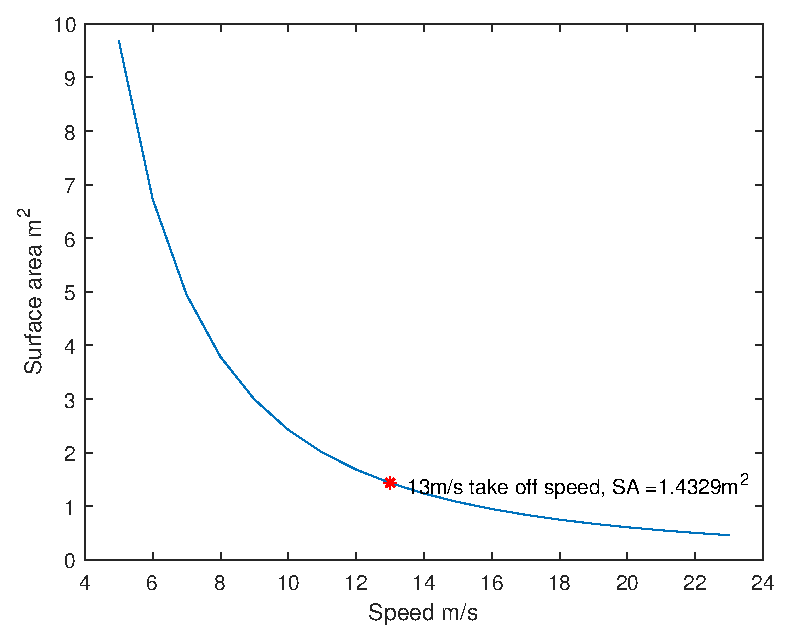
\includegraphics [width=4in]{Plane_Calcs_01.eps}


\subsection*{Drag}

\begin{verbatim}
V = vp*2.5;
cd = .05; %standard drag coefficient of a plane
Drag = cd*take*0.5*d*V^2;
\end{verbatim}


\subsection*{Thrust}

\begin{verbatim}
diam = 12; %prop diameter
pitch = 6; %prop pitch
RPM = 36000;
C1 = 4.392399*10^-8;
C2 = 4.23333*10^-4;

Thrust = C1*RPM*((diam^3.5)/sqrt(pitch))*(C2*RPM*pitch); %source: http://www.electricrcaircraftguy.com/2013/09/propeller-static-dynamic-thrust-equation.html
\end{verbatim}


\subsection*{DATA}

\begin{verbatim}
T_ex = Thrust - Drag;%excess thrust
acc = T_ex/weight%acceleration achievable
dis = (0.3048*170);
TOV = sqrt(2*acc*dis)
time = (2*(dis))/vp;
\end{verbatim}

        \color{lightgray} \begin{verbatim}
acc =

    1.7248


TOV =

   13.3695

\end{verbatim} \color{black}
    


\end{document}
    
